\documentclass{book}

% PACKAGES
%--------------------------------------------------------------------------%
\usepackage[utf8]{inputenc}
\usepackage{tikz}
\usepackage{pgfplots}
\usepackage{wrapfig}

\usepackage{csquotes}
\usepackage{amsmath}
\usepackage{epigraph}
\usepackage[linesnumbered,ruled]{algorithm2e}
\usepackage{adjustbox}

\DeclareMathOperator*{\argmin}{arg\,min} %argmin
\DeclareMathOperator*{\argmax}{arg\,max} %argmax

\usepackage{floatrow}
% Table float box with bottom caption, box width adjusted to content
\newfloatcommand{capbtabbox}{table}[][\FBwidth]
\usepackage{caption}
\usepackage{subcaption}
\captionsetup{compatibility=false}

%%%

\usepackage{array}
% For tabulars
\newcolumntype{P}[1]{>{\centering\arraybackslash}p{#1}}


\usepackage{pdfpages}
\usepackage{graphicx}
\usepackage{longtable}
%\usepackage[export]{adjustbox}
%\usepackage{tabu}
\usepackage{xcolor,colortbl}
\usepackage{caption}
\usepackage{subcaption}
\usepackage{float}
\usepackage{wrapfig}
\usepackage{amsfonts}

% LOAD CUSTOM COMMANDS FROM A FILE
%--------------------------------------------------------------------------%
%\usepackage{result_figures}


% TITLE
%--------------------------------------------------------------------------%


\author{Jakub Ciecierski}
\date{\today}



% DOCUMENT
%--------------------------------------------------------------------------%

\begin{document}


\begin{titlepage}
    \begin{center}

            \textbf{\Huge Projektowanie Systemów CAD/CAM} \\ {\huge Cloud Fitting.} \\ [0.5cm]

            \vspace*{\fill}

            \textbf{\large Jakub Ciecierski \\ Anna Witwicka \\ Lukasz Wójcik}

            \vspace*{\fill}
            
            \textnormal{\large Warsaw University of Technology \\ Factulty of Mathematics and Information Science. \\ \today}

    \end{center}
\end{titlepage}

\tableofcontents


%---------------------------------------------------------------
\chapter{Particle Swarm Optimization}\label{chap:pso}

The Particle Swarm Optimization (PSO) is population based stochastic optimization algorithm, originated by Eberhart and Kennedy~\cite{pso_origin}. Swarm of particles fly through the search space in order to find the most optimal solution of a given problem. The particles remember the best found solution and the further search is affected by it.

Each particle consists of the several fields. The position $X_p$ and velocity vector $V_p$ lets the particle travel through the search space. $Fitness$ value which is evaluated by the fitness function, represents the quality of the solution. The particle also remembers the best fitness value computed so far. Finally, two additional positions called $pbest_p$ and $lbest_p$ are stored. The position in which the particle $p$ reached its best fitness value so far is called $pbest_p$. However, the $lbest_p$ is the position of the best fitness value obtained so far by any other particle in the neighbourhood of particle $p$. The concept of neighbourhood is defined later in this chapter.

PSO is initialized with random group of particles. It then searches for the optimal solution by updating positions of the particles.
In each iteration $t$, the particles are updated by calculating potentially new $pbest_p$ and $lbest_p$ positions which affect the change in current velocity of the particle. $X_p(t)$ will denote the position of particle $p$ at time $t$, i.e. the $t$-th iteration. Similarly, the velocity vector is denoted by $V_p(t)$.

Firstly, the general flow of the PSO algorithm is given, then each functionality is discussed and defined in details.

\begin{center}
    
    \begin{enumerate}
        \item For swarm size s, initialize the group of particles.
        
        \item For each particle: \label{itm:pso_iter}
        \begin{enumerate}
            \item Calculate the fitness value, using the fitness function.
            \item Compare the fitness to its best obtained so far, the better value is stored together with $pbest_p$	
            
            \item Update neighbourhoods and find $lbest_p$ position.
            
            \item Update velocity and position.	
        \end{enumerate}
        
        \item Repeat~\ref{itm:pso_iter}. until maximum number of iterations has been reached.
        
    \end{enumerate}
    
\end{center}



%The remaining part of this chapter is devoted to illustrating problems associated with the objective of this study and more importantly, methods of solving these problems.


%---------------------------------------------------------------------
%---------------------------------------------------------------------
\section{Swarm Initialization}
In order to initialize the PSO algorithm, one must first decide on the size of the swarm (i.e. the number of particles). The swarm will be a static group, meaning that the size will not change through out the computations of a single PSO instance.

The interval for position of all particles must also be chosen. The interval along with the size of the position will essentially define the search space for the swarm.

Additionally, it is convenient to define a constant $v_{max}$ which prevents the particle from traveling in any dimension, further than $v_{max}$ distance in a single iteration. If the velocity was not limited, the jumps in position between iterations could be quite big. This could lead the particles to avoid a big chunk of the search space.


%---------------------------------------------------------------------
%---------------------------------------------------------------------
\section{Neighbourhood}

The neighbourhoods are updated using a simply algorithm based on star topology.
For each particle, neighbourhood is created containing itself and $K$ other random particles. Among that neighbourhood the best particle is found which defines the $lbest$ of the particle of interest.

The neighbourhoods are updated only when there was no change in global best (among all particles in the swarm) since the last iteration.


%---------------------------------------------------------------------
%---------------------------------------------------------------------
\section{Updating the particle}


The following method of updating the particles has its origins in the Standard Particle Swarm Optimization version 2011 presented in~\cite{pso_11}

Let $G_p(t)$ be the centre of gravity of the three points:
\begin{enumerate}
    \item Current position. \\
    $X_p(t)$
    
    \item Point a bit beyond $pbest_p$. \\
    $Y_{p1}(t) = c(pbest_p-X_p(t))$
    
    \item Point a bit beyond $lbest_p$. \\
    $Y_{p2}(t) = c(lbest_p-X_p(t))$
    
\end{enumerate}

The constant $c = \frac{1}{2} + ln(2)$ called a learning factor, together with the inertia parameter that weights the particle's velocity $\omega = \frac{1}{2 * ln(2)}$ used in further equations, was proposed by Clerc in~\cite{pso_anal}.

Formally $G_p(t)$ it is defined by the following formula 
\begin{equation}
G_p(t) = \frac{X_p(t) + Y_{p1}(t) + Y_{p2}(t)} {3}
\end{equation}

We now define a random point $X^{'}_p$ in the hypersphere
\begin{center}
    $\mathcal{H}_p(G_p, d(G_p, X_p))$ 
\end{center}
of centre $G_p$ and of radius $d(G_p, X_p)$ where the function $d$ is an euclidean distance between two points. The time $t$ has been omitted for simplicity.

The velocity update is computed by
\begin{equation}
V_p(t+1) = \omega  V_p(t) + X^{'}_p(t) - X_p(t)
\end{equation}
Thus the position is updated by the equation

\begin{equation}
X_p(t+1) = \omega  V_p(t) + X^{'}_p(t)
\end{equation}

Figure~\ref{fig:pso_sphere} illustrates the idea of updating the position.

\begin{figure}[H]
    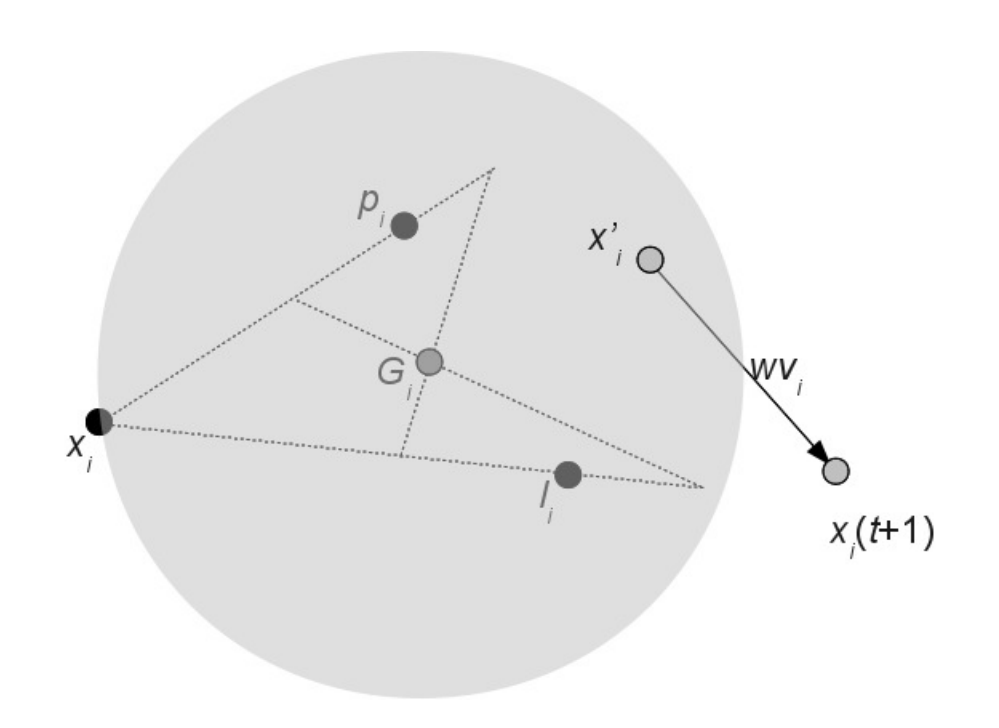
\includegraphics[width=0.7\textwidth]{./images/pso_sphere.png}
    \caption{Example of sphere  $\mathcal{H}_p(G_p, d(G_p, X_p))$. Point $x^{'}_{i}$ is chosen randomly within the sphere}
    \label{fig:pso_sphere}
\end{figure}

% Interval confinement
It may happen that the particle might leave the search space, in means that the particle lies outside the acceptable interval. If that happens we generally try to lead the particle back to its right course. For each dimension $x_{d} \in X_p$ that lies  outside the acceptable interval we apply the following:

\[
x_{d} \notin [x_{min}, x_{max}] \Rightarrow \left \{
\begin{array}{ll}
v_{d} = 0 \\
x_d < x_{min} \Rightarrow x_d = x_{min} \\
x_d > x_{max} \Rightarrow x_d = x_{max}
\end{array}
\right.
\]

This means that the corresponding dimension of velocity vector $v_d \in V_p$ is zeroed and the position is bound to the edge of the interval.

\section{Applying PSO}
In order to implement PSO for problem of interest, one must provide specific implementation for two major components of the algorithm. The first one is fitness function which optimizes the solution to a certain goal. The second one is particle representation method allowing to decode the particle into a specific object which can then be used in the fitness function.

\chapter{Gradient Descend}
Another Algorithm we can use to fit a cloud of points to an object of interest is Gradient Descend. Gradient Descend finds a local minimum of a given goal function. It is one of the simplest iterative optimization algorithm. We find a local minimum by taking steps proportional to the negative of the gradient of a function at the current point.

%---------------------------------------------------------------------
%---------------------------------------------------------------------
\section{Description}
First of all the goal function $f:D \rightarrow \mathbb{R}$ where $D \subset \mathbb{R}^n$ must be defined and differentiable: $f \in C^1$.
For a given goal function we then choose a starting point $x_0 \in D$ and calculate search direction $d_k \in D$ at $x_0$. Next we calculate point at the next step $x_{k+1}$ according to the formula: $$x_{k+1} = x_k + a_k \cdot d_k$$
We check if the stop condition is satisfied. If it is not we repeat whole procedure from the begging. 
\\
\\
In Gradient Descend algorithm \textbf{searching direction $d_k$} is a negative gradient of a goal function $-\nabla f(x_k)$ whereas \textbf{factor $a_k$} corresponds to the length of a step along the negative of the gradient. Step $a_k$ should be relatively small. If the search condition won't be satisfied we can also repeat the procedure with the smaller value of $a_k$.
\\
\\ 
To check if the point $x_k$ is a good approximation of a local minimum, we can check for the following \textbf{stop conditions}:
\begin{itemize}
\item $\Vert \nabla f(x_k \Vert \leq \varepsilon$
\item $\Vert x_{k+1} - x_k \Vert$
\end{itemize}

%---------------------------------------------------------------------
%---------------------------------------------------------------------
\section{Algorithm}
The whole algorithm can be written in the following steps:
\begin{enumerate}
\item Choose the starting point $x_0$
\item $x_{k+1} = x_k + a_k \cdot d_k$
\item Check for Stop Condition
\item If $f(x_{k+1}) \geq f(x_k)$ then decrease the value of $a_k$ and go back to $2.$
\item Repeat from $2.$ for the next step $k+1$
\end{enumerate}

%---------------------------------------------------------------------
%---------------------------------------------------------------------
\section{Construction of the goal function}
The goal function will minimize distances between points in the cloud and the sphere. It will also minimize differences between normals of the points in the cloud and normals on the sphere, so the cloud of points can be appropriately rotated to suit the sphere.  

We will define our goal function as $F(dT, \omega)$ were $dT$ is a 3 dimensional translation and $\omega$ is a rotation (also in 3 dimentions) of the clound of points. Function that finds the closest point on the surface of the sphere in respect to a point in the cloud, will be denoted by $f(p_i)$
$$F(dT, \omega) = \alpha_d \cdot \sum_{i=1}^{k}(\Vert p_i-f(p_i) \Vert)^2 + \alpha_n \cdot \sum_{i=1}^{k}(1-n_i \bullet N_i)$$
where $k$ is a number of points in the cloud, $\alpha_d, \alpha_n$ - constants denoting weights of terms in the equation, $p_i$ - position of the i\textsuperscript{th} point in the cloud, $n_i$ - normal of the i\textsuperscript{th} point in the cloud, $N_i$ - normal of the point on the sphere which is closest to the i\textsuperscript{th} point in the cloud.

Due to the dot product $(1-n_i \bullet N_i)$ being subtracted from $1$, the goal function will be minimal as $n_i$ and $N_i$ are more parallel to each other. We also use the euclidean distance to minimize distances between points.

%---------------------------------------------------------------------
%---------------------------------------------------------------------
\section{Computing the gradient}

From our previous goal function formula we can now calculate it's gradient. Let $p_i-f(p_i)$ be denoted by $dist_i$.
$$dF(dT, \omega) = 2\cdot \alpha_d \cdot \sum_{i=1}^{k}dist_i \cdot d_{p_i} \cdot \frac{\partial f(p_i)}{\partial p_i} - \alpha_n \cdot \sum_{i=1}^{k}(n_idN_i + dn_iN_i)$$
where: 
\\derivative of a position of a point in the cloud can be expressed as a dot product of it's 'current rotation' $(p_i - \Theta)$ with $\omega$ and a translation by $dT$:
$$d_{p_i} = \omega \bullet (p_i - \Theta) + dT = \omega \bullet PO + dT =
\begin{bmatrix}
	dT_x + \omega_y\cdot PO_z - \omega_z\cdot PO_y\\
	dT_y - \omega_x\cdot PO_z + \omega_z\cdot PO_x\\
	dT_z + \omega_x\cdot PO_y - \omega_y\cdot PO_x
\end{bmatrix}$$
similarly derivative of a normal of a point in the cloud is a change in it's rotation:
$$d_{n_i} = \omega \bullet (p_i - \Theta) = 
\begin{bmatrix}
	\omega_y\cdot PO_z - \omega_z\cdot PO_y\\
	- \omega_x\cdot PO_z + \omega_z\cdot PO_x\\
	\omega_x\cdot PO_y - \omega_y\cdot PO_x
\end{bmatrix}$$
derivative of a position of a point on the sphere is equal to the normal to the surface at this point:
$$\frac{\partial f(p_i)}{\partial p_i} = N_i =
\begin{bmatrix}
	F_x\\
	F_y\\
	F_z
\end{bmatrix}$$
derivative of a normal of a point on the sphere doesn't change between iterations and thus will be equal to 0:
$$d_{N_i} = 0$$

Hence we can further write:

$$dF(dT.x, dT.y, dT.z, \omega_x, \omega_y, \omega_z)$$
$$ = 2\cdot \alpha_d \cdot \sum_{i=1}^{k}dist_i \cdot 
\begin{bmatrix}
	dT_x + \omega_y\cdot PO_z - \omega_z\cdot PO_y\\
	dT_y - \omega_x\cdot PO_z + \omega_z\cdot PO_x\\
	dT_z + \omega_x\cdot PO_y - \omega_y\cdot PO_x
\end{bmatrix}
\cdot 
\begin{bmatrix}
	F_x\\
	F_y\\
	F_z
\end{bmatrix}
-\alpha_n \cdot \sum_{i=1}^{k}
\begin{bmatrix}
	\omega_y\cdot PO_z - \omega_z\cdot PO_y\\
	- \omega_x\cdot PO_z + \omega_z\cdot PO_x\\
	\omega_x\cdot PO_y - \omega_y\cdot PO_x
\end{bmatrix} \bullet N_i$$


\chapter{Interface}

Figure~\ref{fig:gui1} shows the interface after the application is started. In order to add an object, open the Object Menu by clicking the button in the top right corner as shown in figure~\ref{fig:gui2}. Choose \textit{Sphere} and press \textit{OK}, figure~\ref{fig:gui3}. Then Select the sphere and right click in the Scene tree and choose \textit{Create Cloud}, figure~\ref{fig:gui6}. To start cloud fitting computations, select both Sphere and Cloud, right click and choose the algorithm of choice.

\begin{figure}[H]
    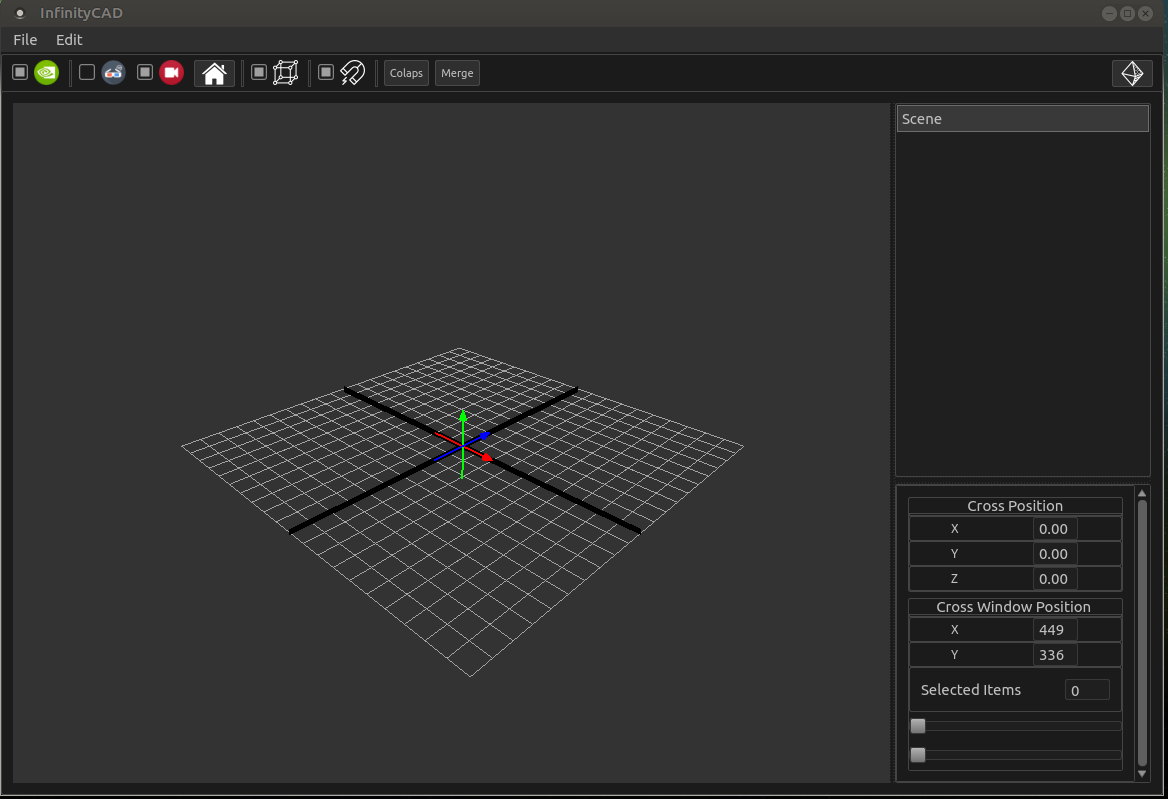
\includegraphics[width=1\textwidth]{./graphics/gui/gui1.png}
    \caption{Application after start up}
    \label{fig:gui1}
\end{figure}

\begin{figure}[H]
    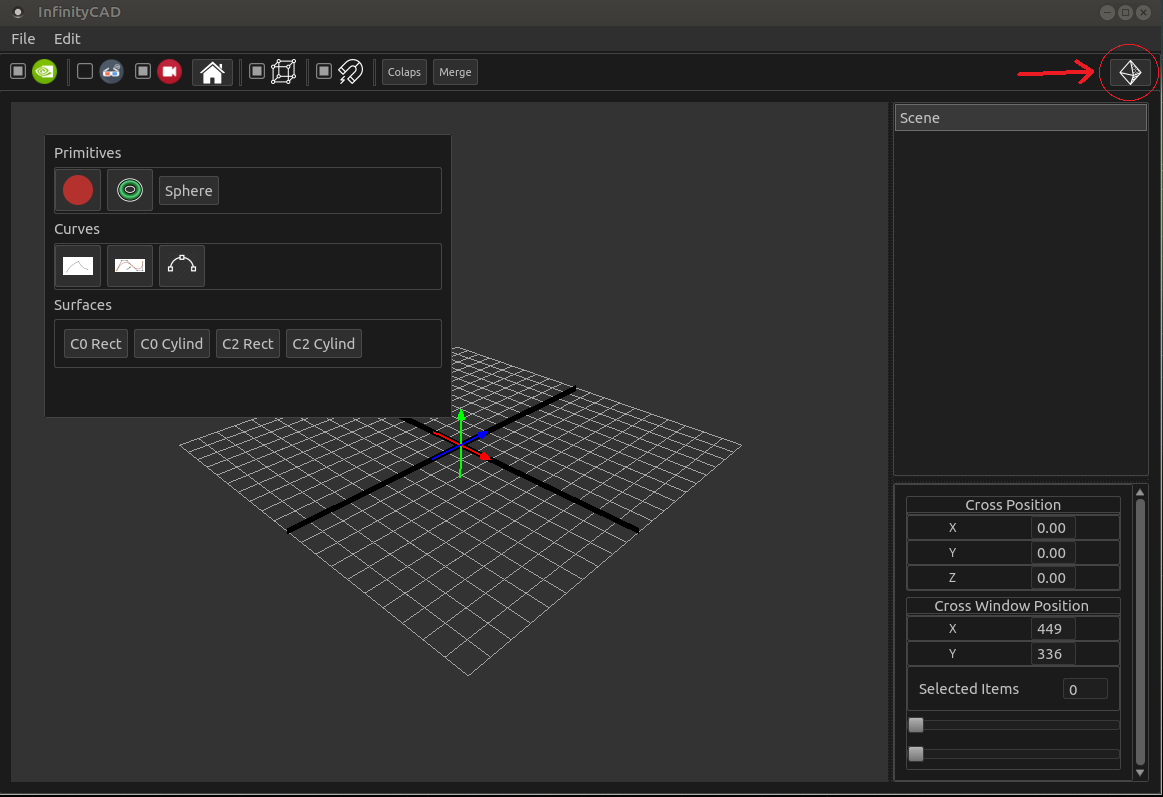
\includegraphics[width=1\textwidth]{./graphics/gui/gui2.png}
    \caption{Object Menu}
    \label{fig:gui2}
\end{figure}

\begin{figure}[H]
    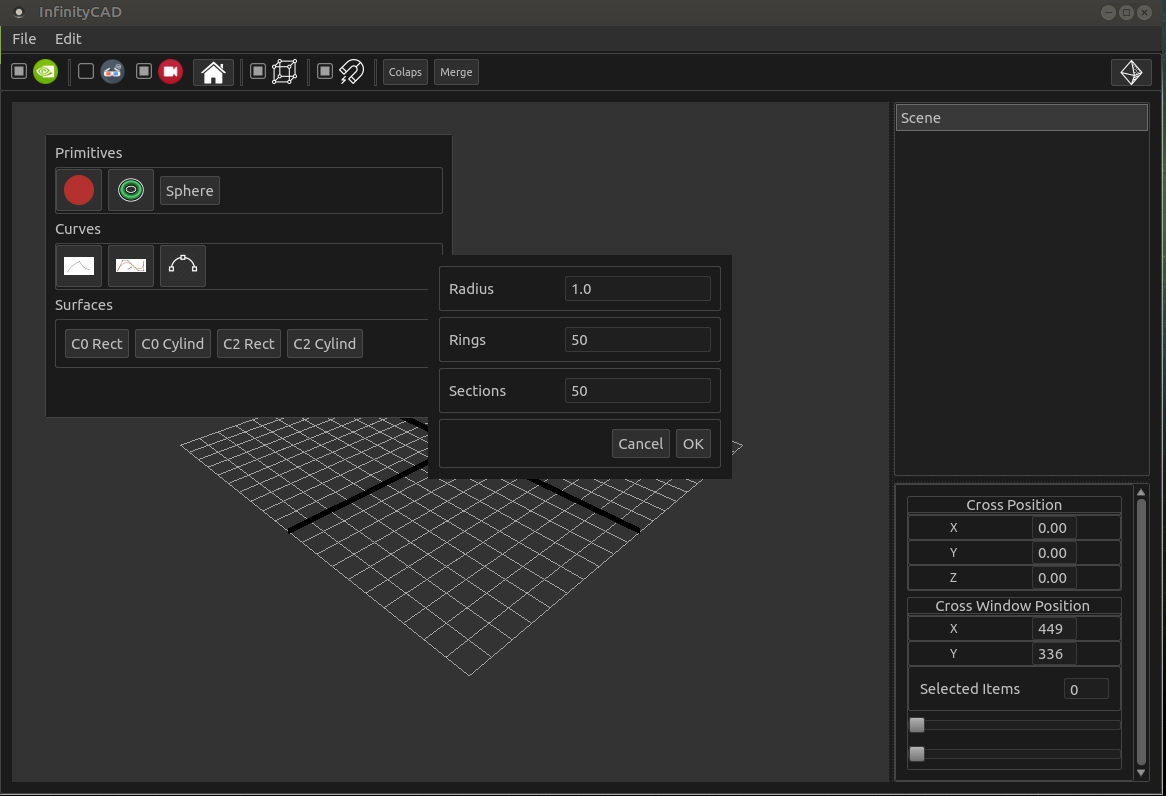
\includegraphics[width=1\textwidth]{./graphics/gui/gui3.png}
    \caption{Creating Sphere}
    \label{fig:gui3}
\end{figure}

\begin{figure}[H]
    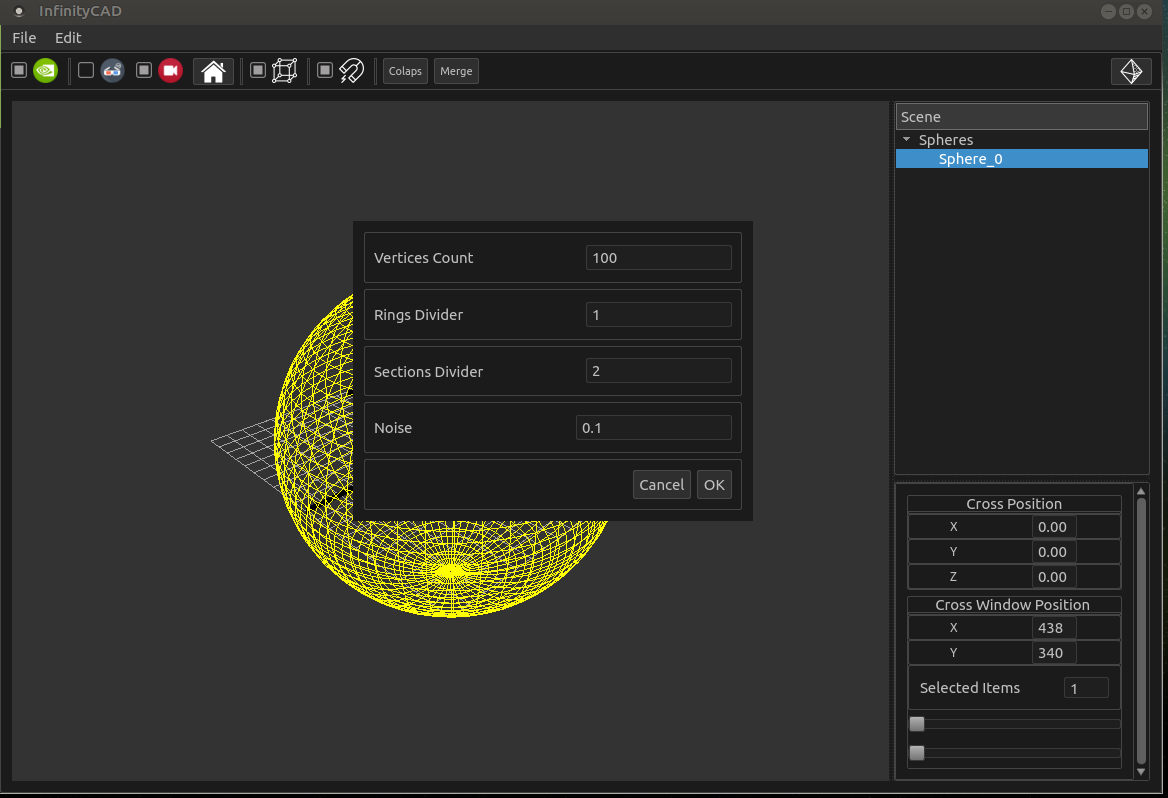
\includegraphics[width=1\textwidth]{./graphics/gui/gui6.png}
    \caption{Extracting Cloud}
    \label{fig:gui6}
\end{figure}

\begin{figure}[H]
    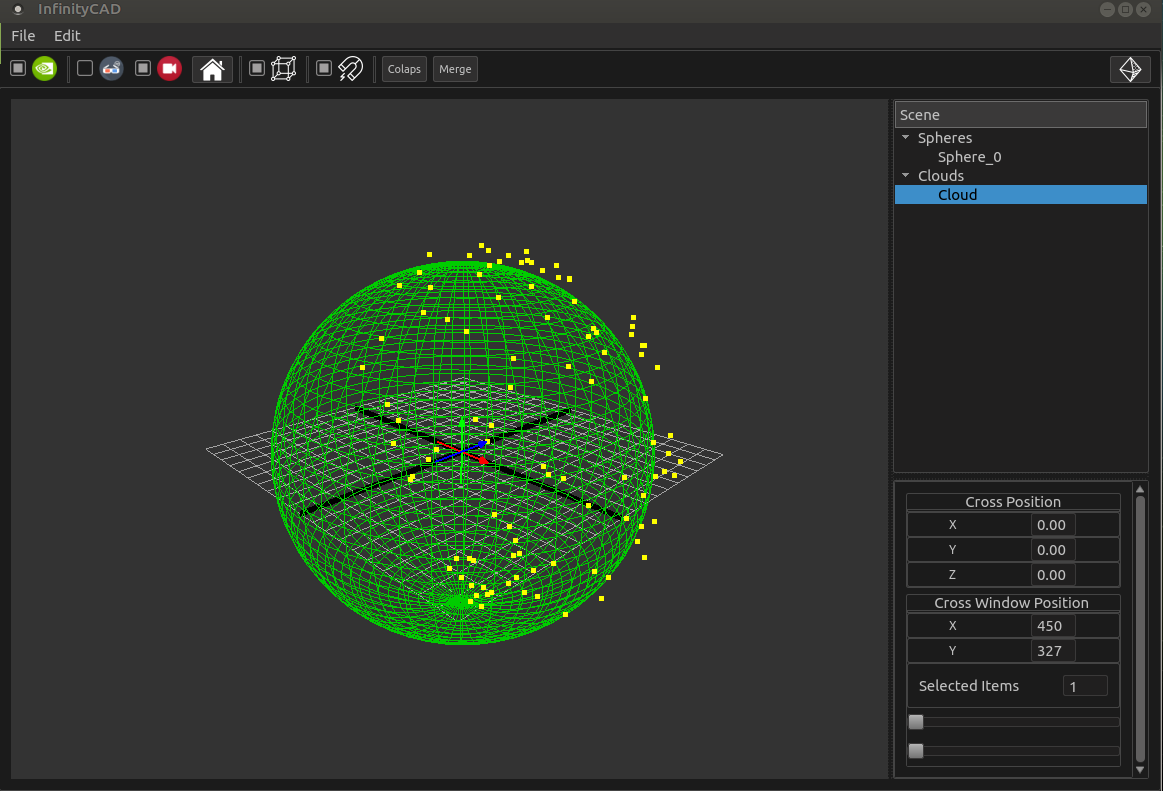
\includegraphics[width=1\textwidth]{./graphics/gui/gui7.png}
    \caption{Cloud}
    \label{fig:gui7}
\end{figure}


\end{document}
